% Standalone TikZ for Figure 3: Shadow Map & Signed Image Header (clean, no overlap)
\documentclass[border=15pt]{standalone}
\usepackage{tikz}
\usetikzlibrary{shapes.geometric, positioning, arrows.meta, patterns, calc}
\definecolor{vbfcBlue}{HTML}{1B4F72}
\definecolor{vbfcDarkBlue}{HTML}{0D2B40}
\definecolor{vbfcAccent}{HTML}{E86C00}
\definecolor{vbfcLightGray}{HTML}{F2F2F2}
\definecolor{vbfcMediumGray}{HTML}{CCCCCC}
\definecolor{vbfcDarkGray}{HTML}{555555}
\definecolor{vbfcOrange}{HTML}{F39C12}
\definecolor{vbfcGreen}{HTML}{27AE60}
\definecolor{vbfcTeal}{HTML}{16A085}
\definecolor{vbfcPurple}{HTML}{8E44AD}
\definecolor{vbfcRed}{HTML}{C0392B}
\begin{document}
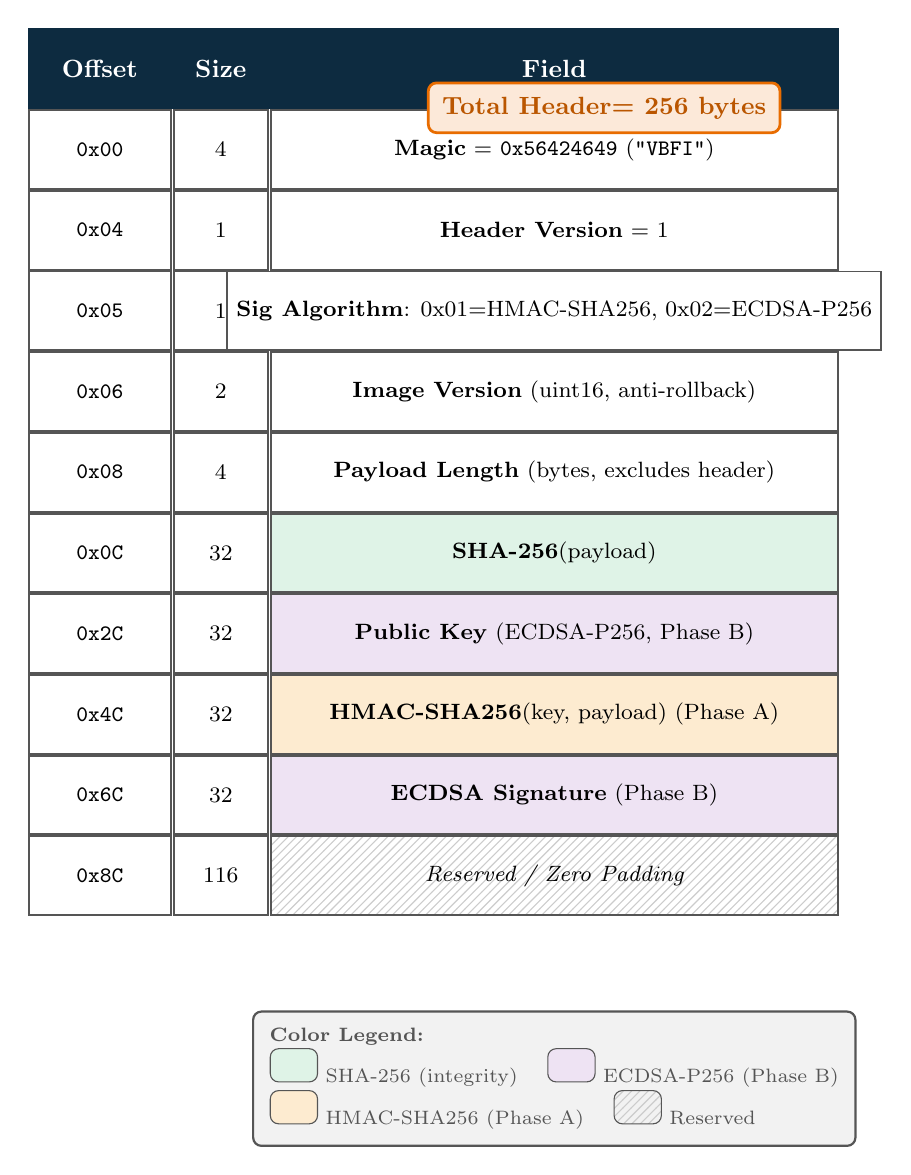
\begin{tikzpicture}[
    node distance=0pt,
    hdr/.style={
        draw=vbfcDarkBlue, line width=1pt, minimum height=10mm,
        fill=vbfcDarkBlue, font=\small\bfseries, text=white,
        anchor=center
    },
    fld/.style={
        draw=vbfcDarkGray, line width=0.7pt, minimum height=10mm,
        fill=white, font=\footnotesize, anchor=center, align=left
    },
    phfld/.style={
        draw=vbfcDarkGray, line width=0.7pt, minimum height=10mm,
        fill=vbfcLightGray, font=\footnotesize\itshape, anchor=center, align=center,
        pattern=north east lines, pattern color=vbfcMediumGray
    },
    crc/.style={
        draw=vbfcDarkGray, line width=0.7pt, minimum height=10mm,
        fill=vbfcGreen!15, font=\footnotesize, anchor=center, align=left
    },
    hmac/.style={
        draw=vbfcDarkGray, line width=0.7pt, minimum height=10mm,
        fill=vbfcOrange!20, font=\footnotesize, anchor=center, align=left
    },
    ecdsa/.style={
        draw=vbfcDarkGray, line width=0.7pt, minimum height=10mm,
        fill=vbfcPurple!15, font=\footnotesize, anchor=center, align=left
    },
    offstyle/.style={font=\scriptsize, text=vbfcMediumGray, anchor=east}
]

% === Header table ===
% Row 0: Headers
\node[hdr, minimum width=18mm] (h_off) {Offset};
\node[hdr, minimum width=12mm, right=of h_off] (h_sz) {Size};
\node[hdr, minimum width=72mm, right=of h_sz] (h_fld) {Field};

% Row 1: 0x00, 4, Magic
\node[fld, minimum width=18mm, below=of h_off] (o00) {\texttt{0x00}};
\node[fld, minimum width=12mm, below=of h_sz] (s00) {4};
\node[fld, minimum width=72mm, below=of h_fld] (f00) {\textbf{Magic} = \texttt{0x56424649} (\texttt{"VBFI"})};

% Row 2: 0x04, 1, Header Version
\node[fld, minimum width=18mm, below=of o00] (o04) {\texttt{0x04}};
\node[fld, minimum width=12mm, below=of s00] (s04) {1};
\node[fld, minimum width=72mm, below=of f00] (f04) {\textbf{Header Version} = 1};

% Row 3: 0x05, 1, Sig Algorithm
\node[fld, minimum width=18mm, below=of o04] (o05) {\texttt{0x05}};
\node[fld, minimum width=12mm, below=of s04] (s05) {1};
\node[fld, minimum width=72mm, below=of f04] (f05) {\textbf{Sig Algorithm}: 0x01=HMAC-SHA256, 0x02=ECDSA-P256};

% Row 4: 0x06, 2, Image Version
\node[fld, minimum width=18mm, below=of o05] (o06) {\texttt{0x06}};
\node[fld, minimum width=12mm, below=of s05] (s06) {2};
\node[fld, minimum width=72mm, below=of f05] (f06) {\textbf{Image Version} (uint16, anti-rollback)};

% Row 5: 0x08, 4, Payload Length
\node[fld, minimum width=18mm, below=of o06] (o08) {\texttt{0x08}};
\node[fld, minimum width=12mm, below=of s06] (s08) {4};
\node[fld, minimum width=72mm, below=of f06] (f08) {\textbf{Payload Length} (bytes, excludes header)};

% Row 6: 0x0C, 32, SHA-256(payload)
\node[fld, minimum width=18mm, below=of o08] (o0c) {\texttt{0x0C}};
\node[fld, minimum width=12mm, below=of s08] (s0c) {32};
\node[crc, minimum width=72mm, below=of f08] (f0c) {\textbf{SHA-256}(payload)};

% Row 7: 0x2C, 32, Public Key (Phase B)
\node[fld, minimum width=18mm, below=of o0c] (o2c) {\texttt{0x2C}};
\node[fld, minimum width=12mm, below=of s0c] (s2c) {32};
\node[ecdsa, minimum width=72mm, below=of f0c] (f2c) {\textbf{Public Key} (ECDSA-P256, Phase B)};

% Row 8: 0x4C, 32, HMAC
\node[fld, minimum width=18mm, below=of o2c] (o4c) {\texttt{0x4C}};
\node[fld, minimum width=12mm, below=of s2c] (s4c) {32};
\node[hmac, minimum width=72mm, below=of f2c] (f4c) {\textbf{HMAC-SHA256}(key, payload) (Phase A)};

% Row 9: 0x6C, 32, ECDSA Signature (Phase B)
\node[fld, minimum width=18mm, below=of o4c] (o6c) {\texttt{0x6C}};
\node[fld, minimum width=12mm, below=of s4c] (s6c) {32};
\node[ecdsa, minimum width=72mm, below=of f4c] (f6c) {\textbf{ECDSA Signature} (Phase B)};

% Row 10: 0x8C, 116, Reserved
\node[fld, minimum width=18mm, below=of o6c] (o8c) {\texttt{0x8C}};
\node[fld, minimum width=12mm, below=of s6c] (s8c) {116};
\node[phfld, minimum width=72mm, below=of f6c] (f8c) {Reserved / Zero Padding};

% Total header size annotation
\node[draw=vbfcAccent, line width=1pt, rounded corners=3pt, fill=vbfcAccent!15,
      font=\small\bfseries, text=vbfcAccent!80!black, anchor=west, inner sep=5pt]
      at ($(h_sz.east)+(20mm,-5mm)$) {Total Header\\= 256 bytes};

% Phase legend
\node[draw=vbfcDarkGray, line width=0.8pt, rounded corners=3pt, fill=vbfcLightGray,
      font=\scriptsize, text=vbfcDarkGray, anchor=north, inner sep=6pt, align=left]
      at ($(f8c.south)+(0mm,-12mm)$) {
    \textbf{Color Legend:}\\
    \tikz\node[draw,fill=vbfcGreen!15,minimum height=3mm,minimum width=6mm]{};~SHA-256 (integrity) \quad
    \tikz\node[draw,fill=vbfcPurple!15,minimum height=3mm,minimum width=6mm]{};~ECDSA-P256 (Phase B)\\
    \tikz\node[draw,fill=vbfcOrange!20,minimum height=3mm,minimum width=6mm]{};~HMAC-SHA256 (Phase A) \quad
    \tikz\node[draw,pattern=north east lines, pattern color=vbfcMediumGray,minimum height=3mm,minimum width=6mm]{};~Reserved
};

\end{tikzpicture}
\end{document}
